\chapter{Ejercicio 1}

\section{Actividad 1}

\textbf{Actividad 1}. Dada la secuencia de senales {$\phi_{n} (t)=e^{j(n\omega)t}: n \in \mathbb{Z}$}, con $T = \dfrac{2\pi}{\omega}$. Demostrar:

\subsection{A}

\textbf{A)} El periodo fundamental de la senal $\phi_{n}(t)$ es $T_n=\dfrac{2\pi}{n\omega}$. ¿Por qué se puede afirmar que la suma entre estas señales está bien definida $\phi_{n}(t)$?

\textbf{i.} Lo primero que realizaremos seria corroborar que $T_n$ es un periodo.

$$\phi_{n}(t+T_n)=\phi_{n}(t)$$

$$e^{jn\omega(t+T_n)}=e^{jn\omega(t)}$$

$$e^{jn\omega(t+\dfrac{2\pi}{n\omega})}=e^{jn\omega(t)}$$

$$e^{jn\omega(t)+jn\omega\dfrac{2\pi}{n\omega}}=e^{jn\omega(t)}$$

$$e^{jn\omega(t)+j2\pi}=e^{jn\omega(t)}$$

$$e^{jn\omega(t)} \cdot e^{j2\pi} = e^{jn\omega(t)}$$

$$e^{jn\omega(t)} \cdot 1 = e^{jn\omega(t)}$$

$$e^{jn\omega(t)} = e^{jn\omega(t)}$$

\textbf{ii.} Para ver que $T_n$ es el periodo fundamental, suponemos que exisite un $T'>0$ con $T'<T_n$, tal que.

$$\phi_n(t+T')=\phi_n(t)$$

Entonces $e^{jn\omega T'} = 1$, por lo que existe $k \in \mathbb{Z}$ tal que

$$n\omega T'= 2\pi k$$

Despejando $n\omega$

$$T'=\dfrac{2\pi k}{n\omega}$$

Donde si $k=0$ entonces $T'=0$, lo cual contradic lo que postulamos al principio que $T'>0$

Si $|k| \ge 1$, entonces

$$T' \ge \dfrac{2\pi}{|n|\omega} = T_{|n|}$$

Lo cual contradice que $T'<T_n$. Por lo tanto no existe $T'\in(0,T_n)$ que sea periodo.

\textbf{iii.}

Ahora bien podemos concluir que la suma $\sum_{n \in \mathbb{Z}} \phi_n(t)$ está bien definida porque todas las señales $\phi_n(t)$ son periódicas con un periodo común $T = \frac{2\pi}{\omega}$ (múltiplo entero de $T_n$). Esto garantiza que la superposición de señales mantenga la periodicidad global.

\vspace{0.5cm}

\subsection{B}

\textbf{B)} Calcular $E_n = (\phi_n(t), \phi_n(t))_T \quad \text{y} \quad (\phi_n(t), \phi_m(t))_T, \quad \forall n,m \in \mathbb{Z}$

Como primer paso definiremos
\[
\langle \phi_n, \phi_m \rangle_T = \frac{1}{T}\int_0^T \phi_n(t)\overline{\phi_m(t)}dt
\]

\textbf{Caso 1: $n = m$}
\begin{align*}
\langle \phi_n, \phi_n \rangle_T &= \frac{1}{T}\int_0^T e^{jn\omega t}e^{-jn\omega t}dt \\
&= \frac{1}{T}\int_0^T 1\,dt = 1 \quad \forall n
\end{align*}

\textbf{Caso 2: $n \neq m$}
\begin{align*}
\langle \phi_n, \phi_m \rangle_T &= \frac{1}{T}\int_0^T e^{j(n-m)\omega t}dt \\
&= \left.\frac{e^{j(n-m)\omega t}}{j(n-m)\omega T}\right|_0^T = 0 \quad \text{(por periodicidad)}
\end{align*}

\vspace{0.5cm}

\subsection{C}

\textbf{C)} La secuencia de señales $\{ \phi_n(t) = e^{j(n\omega)t} : n \in \mathbb{Z} \}$ es base de Fourier.

\textbf{Propiedades requeridas:}
\begin{enumerate}[label=(\roman*)]
\item \textbf{Ortogonalidad}: $\langle \phi_n, \phi_m \rangle_T = \delta_{nm}$ (demostrado en B)
\item \textbf{Completitud}: Cualquier señal $x(t)$ periódica puede expresarse como:
\[
x(t) = \sum_{n=-\infty}^{\infty} C_n \phi_n(t)
\]
\end{enumerate}

\vspace{0.5cm}

\subsection{D}

\textbf{D)} La secuencia de señales $\{ \rho_n^0(t) = \cos(n\omega t) = \tfrac{1}{2}\phi_n(t) + \tfrac{1}{2}\overline{\phi_n(t)} : n \geq 0 \}$ es base de Fourier.

\textbf{Relación con $\phi_n(t)$:}
\[
\cos(n\omega t) = \frac{1}{2}\phi_n(t) + \frac{1}{2}\phi_{-n}(t)
\]

\textbf{Ortogonalidad:}
\[
\langle \rho_n^0, \rho_m^0 \rangle_T = 
\begin{cases}
1 & n = m = 0 \\
\frac{1}{2} & n = m \neq 0 \\
0 & n \neq m
\end{cases}
\]

\vspace{0.5cm}

\subsection{E}

\textbf{E)} La secuencia de señales \[\{ \rho_n^1(t) = \sin(n\omega t) = \tfrac{1}{2j}\phi_n(t) - \tfrac{1}{2j}\overline{\phi_n(t)} : n > 0 \}\] es base de Fourier.

\textbf{Relación con $\phi_n(t)$:}
\[
\sin(n\omega t) = \frac{1}{2j}\phi_n(t) - \frac{1}{2j}\phi_{-n}(t)
\]

\textbf{Ortogonalidad:}
\[
\langle \rho_n^1, \rho_m^1 \rangle_T = 
\begin{cases}
\frac{1}{2} & n = m \\
0 & n \neq m
\end{cases}
\]

\section{Actividad 2}

\textbf{Actividad 2.} Calcular la descomposicion de series $x(t) = \sum_{n \in \mathbb{Z}}$ y $x(t) = a_0 + \sum_{n=1}^{\infty}(a_n \rho_n ^0(t) + b_n \rho_n ^1(t))$ de las siguientes se\~nales. Para luego calcular aproximadamente la energia de la se\~nal usando el teorema de Parseval.

\subsection{Se\~nal sinusoidal rectificada de onda completa}

\begin{figure}[H]
  \centering
  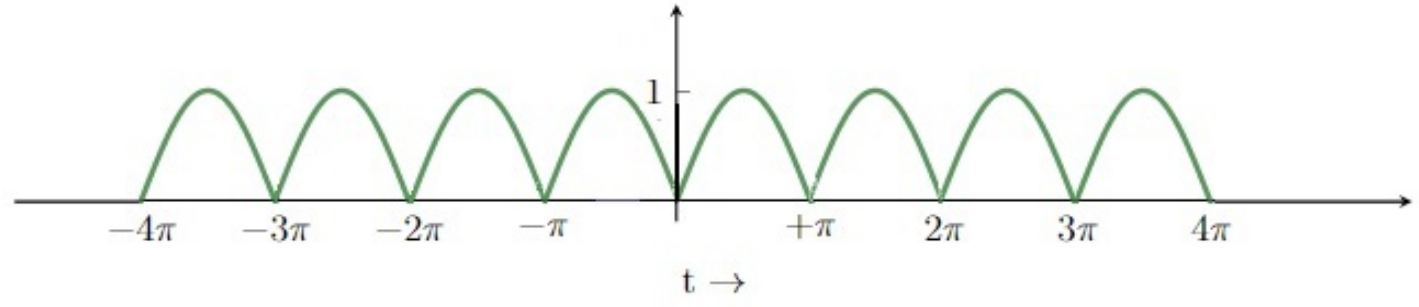
\includegraphics[width=0.8\textwidth]{photos/onda_completa.png}
\end{figure}

La se\~nal se trata de $x(t) = |sen(t)|$.

Primero debemos tomar el periodo de la se\~nal, el cual es igual a $\pi$, para poder calcular el coeficiente $C_n$ el cual esta dado por la siguiente ecuacion.

$$C_n = \dfrac{1}{T} \int_{<T>} x(t) e^{-j(n\omega)t} dt$$

$$C_n = \dfrac{1}{\pi} \int_{0}^{\pi} |sen(t)| e^{-j(n\omega)t} dt$$

Siendo $\omega = \dfrac{2\pi}{T} = 2$

Quedando $e^{-j(n\omega)t} = e^{-j2nt} = cos(2nt)-j\,sen(2nt)$

$$C_n = \dfrac{1}{\pi} \int_{0}^{\pi} |sen(t)| [\cos(2nt) - j sen(2nt)] dt$$

$$C_n = \dfrac{1}{\pi} \bigg[\int_{0}^{\pi} sen(t) cos(2nt) dt + j \int_{0}^{\pi} sen(t) sen(2nt) dt \bigg] $$

Siendo $ \int_{0}^{\pi} sen(t) sen(2nt) dt = 0$

$$C_n = \dfrac{1}{\pi} \bigg[\int_{0}^{\pi} sen(t) cos(2nt) dt + 0 \bigg] $$

Recordando que $sen(A) cos(B) = \dfrac{1}{2} [sen(A+B) + sen(A-B)] $

$$C_n = \dfrac{1}{\pi} \int_{0}^{\pi} \dfrac{1}{2} \bigg[sen(t+2nt)+sen(t-2nt)\bigg] dt $$

$$C_n = \dfrac{1}{\pi}  \dfrac{1}{2} \bigg[\int_{0}^{\pi} sen((1+2n)t) dt + \int_{0}^{\pi}sen((1-2n)t) dt\bigg]$$

$$C_n = \dfrac{1}{2\pi} \bigg[\dfrac{-cos((1+2n)\pi)+cos(0)}{1+2n} + \dfrac{-cos((1-2n)\pi)+cos(0)}{1-2n}  \bigg] $$ 

$$C_n = \dfrac{1}{2\pi} \bigg[\dfrac{-(-1)+1}{1+2n} + \dfrac{-(-1)+1}{1-2n} \bigg]  $$

$$C_n = \dfrac{1}{2\pi} \bigg[\dfrac{2}{1+2n} + \dfrac{2}{1-2n} \bigg] $$

$$C_n = \dfrac{1}{2\pi} \bigg[\dfrac{4}{-4n^2+1}\bigg] $$

$$C_n = -\dfrac{2}{\pi(4n^2+1)}$$

Ahora para escribir la serie recordemos que $\phi_n (t) = e^{j(n\omega)t}$.

$$x(t) = \sum_{n \in \mathbb{Z}} C_n \phi_n (t)$$

$$x(t) = \sum_{n=0}^{\infty} \dfrac{-2}{\pi(4n^2+1)} e^{j2nt} $$

$$x(t) = \dfrac{-2}{\pi} \sum_{n=0}^{\infty} \dfrac{e^{j2nt}}{4n^2+1}$$

Si desarrollamos los primeros terminos de la serie queda

$$x(t) = \dfrac{-2}{\pi} \bigg[1 + \dfrac{e^{j2t}}{5} + \dfrac{e^{j4t}}{17} + \dfrac{e^{j6t}}{37} + ... \bigg] $$

Para expresar la se\~nal en su segunda forma (la cual si es posible ya que la se\~nal con la que estamos trabajando SI es real) nos es de suma importancia saber si la se\~nal es tiene simetria, par, impar o no tiene simetria.

Para que sea par debe cumplir con que $f(-t) = f(t)$, veamos.

$$f(-t) = |sen(-t)| = |-sen(t)| = |sen(t)| = f(t) $$

Por lo que verificamos que la se\~nal es par, entonces

$$b_n = 0 $$

$$a_0 = \dfrac{2}{T} \int_{<\dfrac{T}{2}>} x(t) dt $$

$$a_n = \dfrac{4}{T} \int_{<\dfrac{T}{2}>} x(t) cos \bigg(\dfrac{2n\pi t}{T} \bigg) $$
